This paragraph describes the concept of execution among the system components, which are shown in Figure.~\ref{fig:Component_overview}. Since the relations between system 
components do not change dynamically, this section will describe the execution of a threat being detected.

\paragraph{Threat detected scenario}\mbox{}\\
This scenario unfolds when the sensors detect a missile threat. The sequence diagram shown in figure.~\ref{fig:threatDetectedSeqDia} describes the automatic mode where the system responds without pilot 
interaction.

\begin{figure}[h]
	\centering
	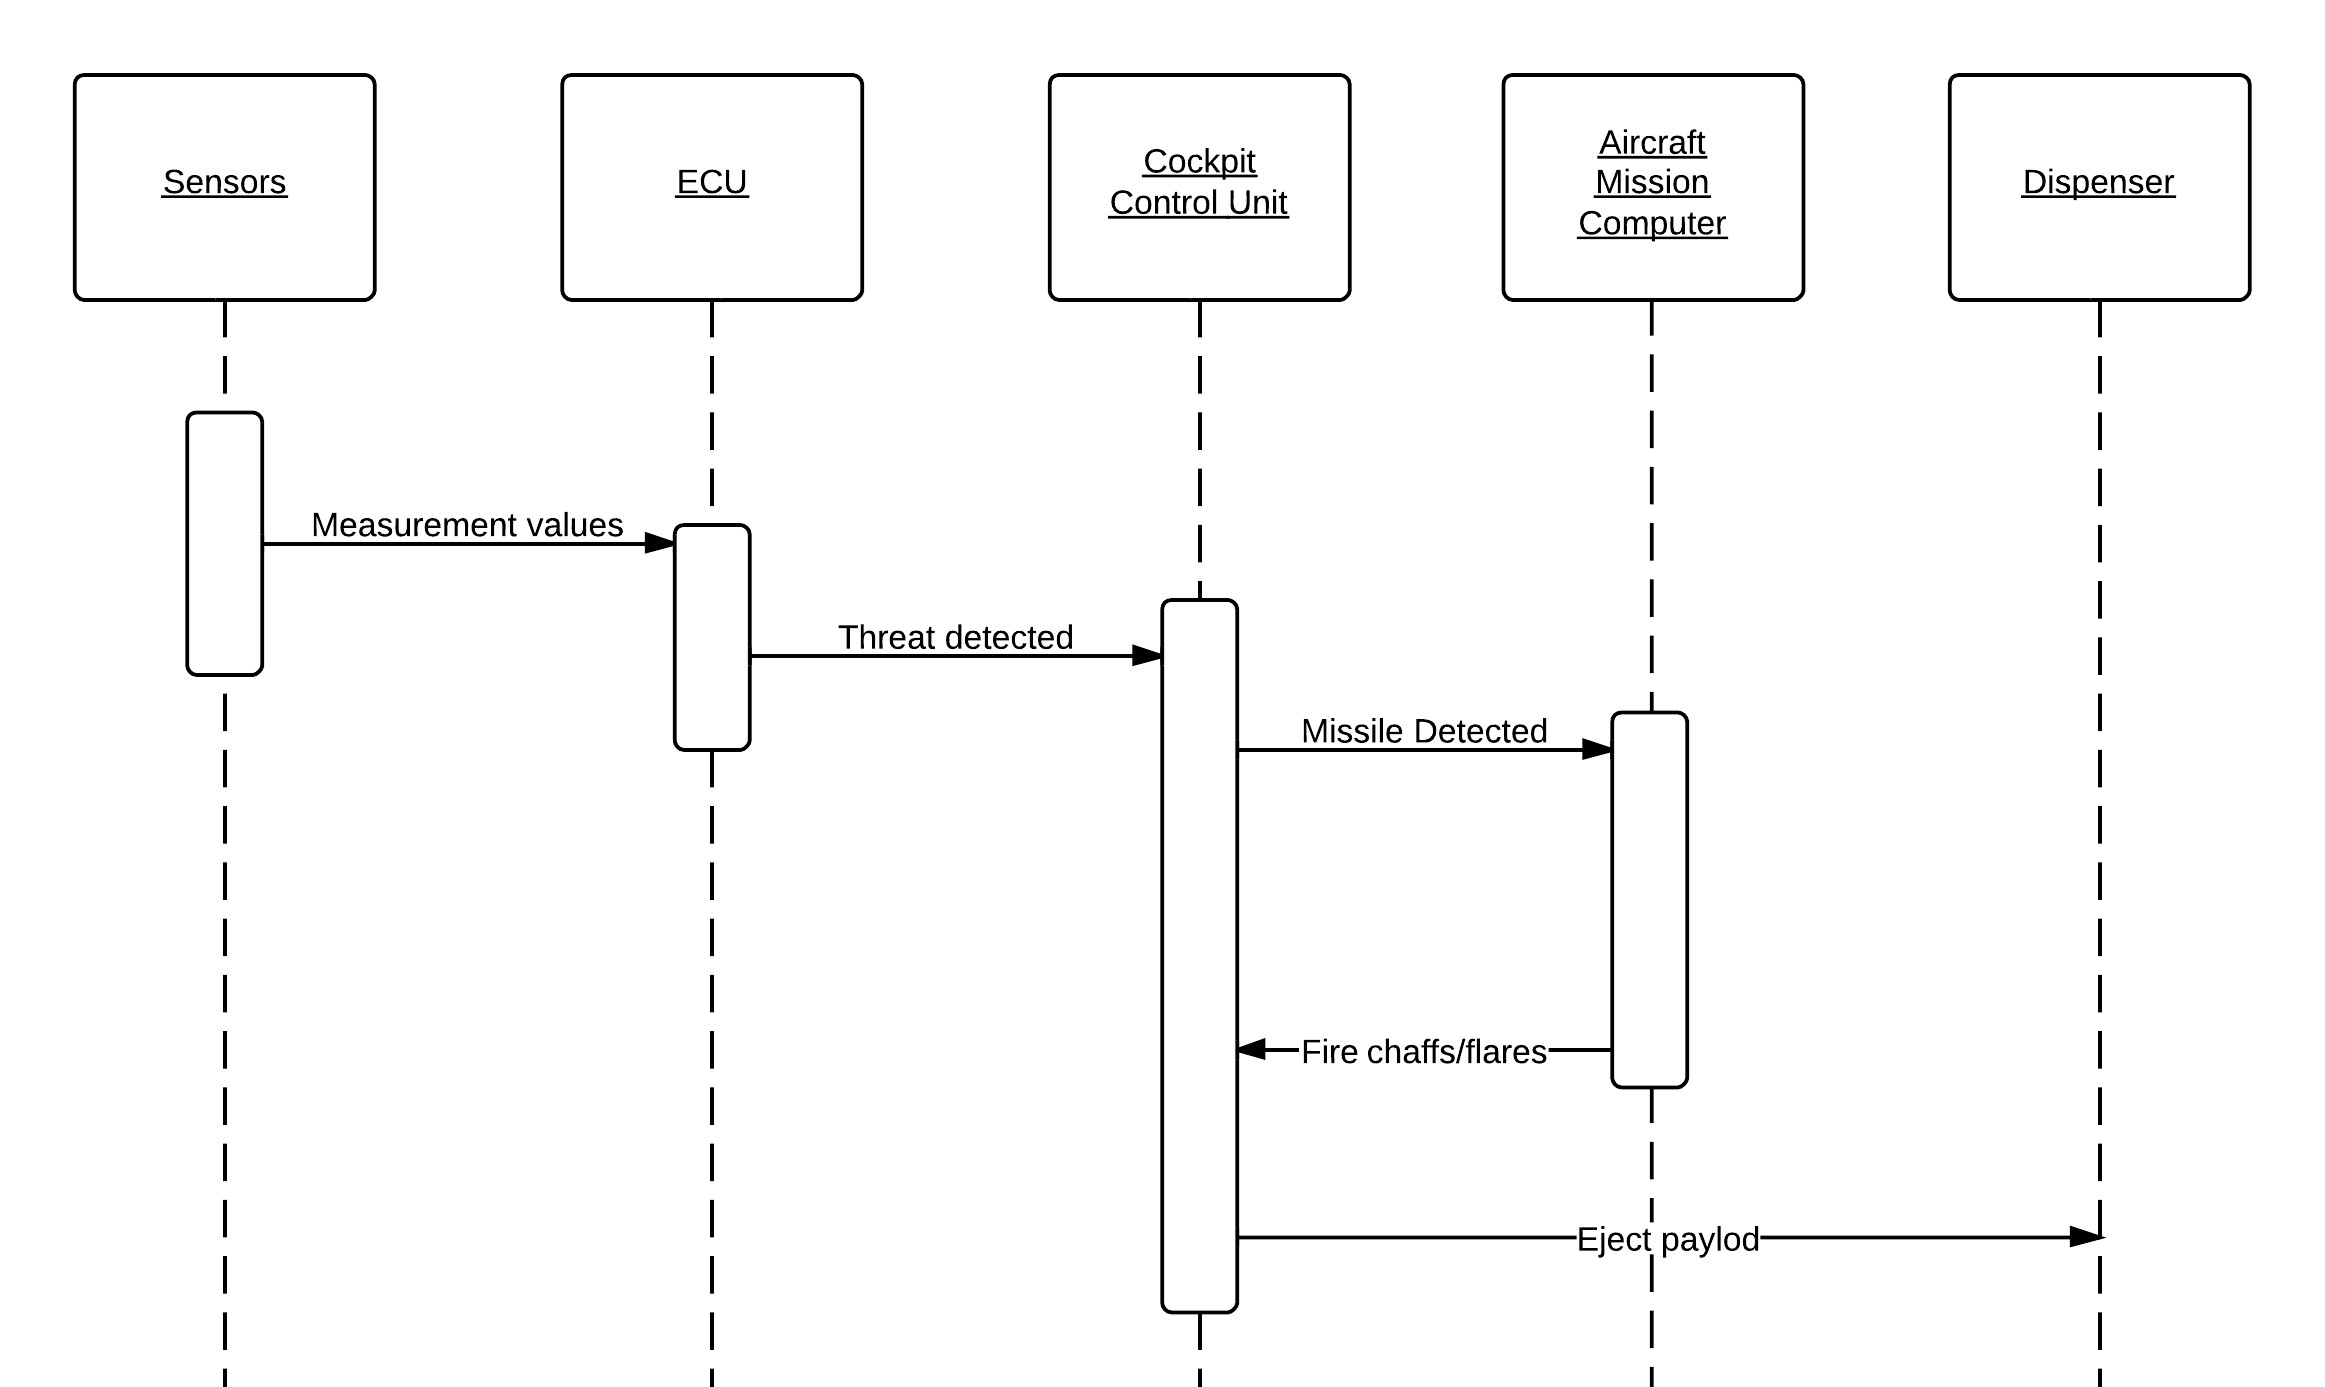
\includegraphics[scale=0.2]{./images/threatDetectedSequenceDiagram.png}\\
	\caption{Threat detected sequence diagram}
    \label{fig:threatDetectedSeqDia}
\end{figure}

